\documentclass[twoside]{article}
\usepackage{../estilo-ejercicios}
\usepackage{tikz}
\usetikzlibrary{automata,positioning}
\newcommand{\x}{{\mathbf{x}}}
\newcommand{\y}{{\mathbf{y}}}
%--------------------------------------------------------
\begin{document}

\title{Procesos Estocásticos. Aplicaciones}
\author{Rafael González López}
\maketitle

\begin{ejercicio}{6}
Una máquina tiene dos piezas colocadas en paralelo de manera que para funcionar utiliza solo una de ellas, quedando la otra de repuesto para reemplazar a la que trabaja cuando esta se estropea, si está en condiciones de trabajar. Las piezas trabajan de manera que se estropean durante un periodo de tiempo dado con una probabilidad $q$. Supongamos que la pieza que está trabajando, en caso de que se estropee, lo hace al final de un periodo, de manera que la pieza de repuesto empieza a trabajar, si está en condiciones de hacerlo, al principio del periodo siguiente. Hay un único mecánico para reparar las piezas estropeadas, que tarda dos periodos en reparar una pieza estropeada. El proceso puede describirse mediante un vector $X_t$ de dos componentes $U$ y $V$, donde $U$ representa el número de piezas hábiles, trabajando o en condiciones de trabajar, al final del periodo $t$-ésimo, y $V$ toma el valor $1$ si el mecánico requiere únicamente un periodos adicional para completar una reparación, si está procediendo a ella, y $0$ en caso contrario. Por lo tanto, el espacio de estados consta de cuatro estados
$$
(2,0), (1,0),(0,1),(1,1)
$$
(Por ejemplo, el estado $(1,1)$ implica que una componente opera y la otra necesita un periodo adicional para acabar de ser reparada). Denotemos los cuatro estados por $0,1,2$ y $3$, respectivamente. (Es decir, $X_t=0$ quiere decir $X_t = (2,0)$, por ejemplo). Se pide:
\begin{itemize}
\item Comprobar que $X_t$ para $t=0,1,\dotsc$ es una cadena de Markov.
\item Describir el diagrama de transiciones y hallar la matriz de probabilidades de transición. 
\end{itemize} 
\end{ejercicio}
\begin{solucion}

\begin{itemize}
\item[]
\item Es claro que el espacio de estados consta de cuatro elementos, luego es discreto. Que se verifica la propiedad de Markov se tiene casi por el propio planteamiento del modelo. El estado futuro de la cadena depende a lo sumo del último estado conocido, pero desde luego no de los anteriores. 
\item El diagrama de trasición es

\begin{center}
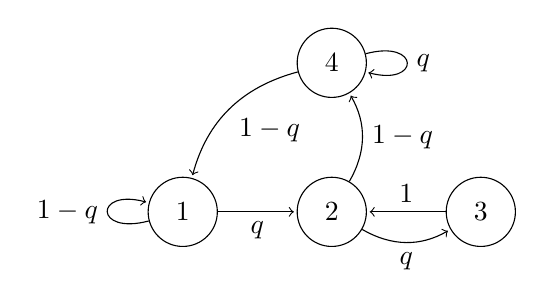
\begin{tikzpicture}
	% Draw the states
	\node[state]             (1) {$1$};
	\node[state, right=of 1] (2) {$2$};
	\node[state, right=of 2] (3) {$3$};
	\node[state, above=of 2] (4) {$4$};
    % Connect the states with arrows
	\draw[every loop]
		(1) edge[right, auto=right] node {$q$} (2)
		(1) edge[loop left] 	   node {$1-q$} (1)
		(2) edge[bend right, auto=right] node {$q$} (3)
		(2) edge[bend right, auto=right] node {$1-q$} (4)
		(3) edge[right, auto=right] node {$1$} (2)
		(4) edge[loop right, auto=left] node {$q$} (3)
		(4) edge[bend right, auto=left] node {$1-q$} (1);
\end{tikzpicture}
\end{center}
La matriz de transición es
$$
\begin{pmatrix}
1-q	& q & 0 & 0\\
0 	& 0	& q	& 1-q\\
0	& 1 & 0 & 0\\
1-q & 0 & 0 & q
\end{pmatrix}
$$
\item Es fácil ver, o bien calculando $P^4$ (es $>0$ y por tanto $P$ es regular) o bien directamente sobre el diagrama, que todos los estados están interconectados cuando $q\in(0,1)$. Por tanto, todos deben tener el mismo carácter. Como estamos en una cadena finita, deben ser todos recurrentes no nulos. Se tiene naturalmente que $f_i = 1$, $i=1,2,3,4$.
\item Que $P$ sea regular implica que la cadena es ergódica. En particular, todos los estados son aperiódicos.
\item Otra consecuencia de que $P$ sea regular es que existe una única distribución límite que además es la distribución estacionaria, luego podemos calcularla directamente.
$$
P =\begin{pmatrix}
1-q	& q & 0 & 0\\
0 	& 0	& q	& 1-q\\
0	& 1 & 0 & 0\\
1-q & 0 & 0 & q
\end{pmatrix} \Rightarrow 
P' =
\begin{pmatrix}
1-q	& 0 & 0 & 1-q\\
q 	& 0	& 1	& 0\\
0	& q & 0 & 0\\
0	& 1-q & 0 & q
\end{pmatrix}
$$
$$
P'-I = 
\begin{pmatrix}
-q	& 0 & 0 & 1-q\\
q 	& -1	& 1	& 0\\
0	& q & -1 & 0\\
0	& 1-q & 0 & q-1
\end{pmatrix}
$$
Resolviendo el sistema e imponiendo que los coeficientes sumen $1$ obtenemos que la distribución estacionaria es
$$
\pi(q) = \sqrt{\frac{q^2}{q^4+3q^2-2q+1}}
\begin{pmatrix}
\dfrac{1-q}{q} & 1 & q & 1
\end{pmatrix}
$$
Está bien definido porque el denominador solo tiene dos raíces reales y son menores que $-1$. Además, es positivo en $[0,1]$.	
\end{itemize}
\end{solucion}
\end{document}